\newpage
\section{Leitner's Box GUI}
\genHeader
\hypertarget{sec:LBGUI}{}

% Uneeded? We talked a little bit about this in injections.. (it adhgeres to metamodel, or type graph)
We would like to now introduce you to the \texttt{Leitner Box Gui}, a small java application generated from your \texttt{.ecore} instance model! This is the
interface where you can interact with your partition and cards and later, once we implement more methods, manipulate the items in your box.

\begin{itemize}

\item[$\blacktriangleright$] Navigate to the top left of your toolbar and select ``New.'' (Fig.~\ref{fig:load_GUI})

\begin{figure}[htbp]
    \centering
    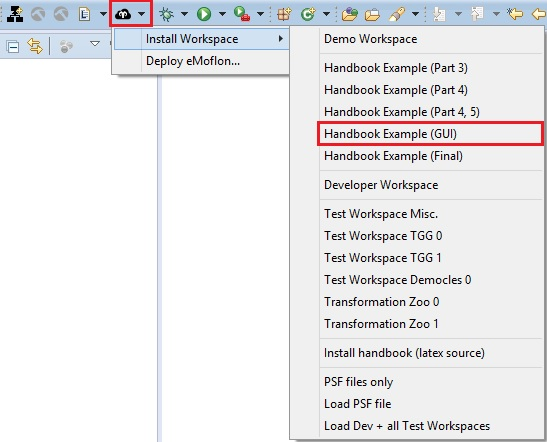
\includegraphics[width=0.7\textwidth]{eclipse_loadGUI}
    \caption{Load Leitner's Box GUI}
    \label{fig:load_GUI}
\end{figure}

\item[$\blacktriangleright$] Load ``Examples/eMoflon Handbook Examples/Leitner Box GUI.'' This will load a new project into your workspace. Right click it to
raise the context menu then select ``Run as/Java application.'' 

\item[$\blacktriangleright$] The program will immediately open to an ``Open File" dialouge. Navigate to and open the \texttt{Box.xmi} instance
file\footnote{If you do not specify a file to open, the GUI will load some default files.}.

\begin{figure}[htbp]
    \centering
    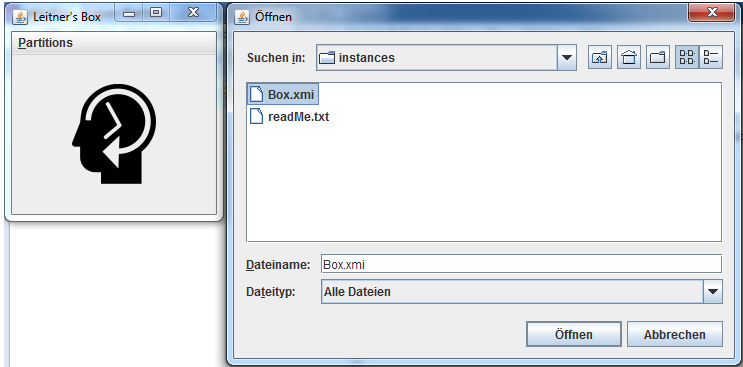
\includegraphics[width=0.8\textwidth]{eclipse_loadXMI}
    \caption{Load the instance file}
    \label{fig:load_XMI}
\end{figure}

\item[$\blacktriangleright$] The main window represents your box, and clicking on the \texttt{Partitions} button will list your current partitions. Hovering
over each element will take you to the next layer in your box.

\item[$\blacktriangleright$] Hover over any card - you should be able to see the \texttt{removeCard} method you implemented via Injections in the previous
section. (Fig.)

\item[$\blacktriangleright$] Experiment with your \texttt{.ecore} model by adding, removing, or renaming more attributes, and observe how they're reflected in
the GUI.

\fancyfoot[R]{ $\triangleright$ \hyperlink{conclusion}{Next}}

\end{itemize}
